%% LatexFile made with sciFxt
\documentclass [11pt,spanish]{article}
\usepackage [spanish,activeacute]{babel}
%\usepackage [latin1]{inputenc}
\usepackage[utf8]{inputenc}
\usepackage { amsmath}
\usepackage { upgreek }
\usepackage { mathrsfs }
\usepackage { graphicx }
\usepackage{subfig}
\usepackage { framed,color }
\setlength {\topmargin}{-.5in}
\setlength {\textheight}{9in}
\setlength {\oddsidemargin}{0in}
\setlength {\textwidth}{6.5in}
\begin {document}
\title {Program report}
\author {MACZ\\
Universidad Nacional Aut\'onoma de M\'exico}
\maketitle 

\graphicspath{{./fig/}}

Túnel circular con recubrimiento. Ambos materiales elásticos e isótropos. Tomado del capítulo 3 de Mow y Pao, "The diffraction of elastic waves and dynamic stress concentrations", 1971. 
Ejercicio para incidencia de onda plana P y SV.

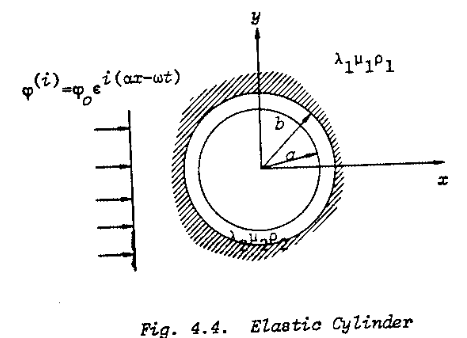
\includegraphics[scale=0.5]{figura}
\begingroup
\fontsize{10pt}{12pt}
\selectfont
\definecolor{shadecolor}{rgb}{0.925,0.925,0.925}
\begin{shaded}
\begin{verbatim}
      module datos
      save
!     real*8, dimension(2), parameter :: rho = (/2.0, 2.0/)
!     real*8, dimension(2), parameter :: nu = (/0.333, 0.333/)
!     real*8, dimension(2), parameter :: bet = (/500.0, 750.0/) !1 medio, 2 liner
      real*8, dimension(2), parameter :: rho = (/2700.0, 7850.0/)
      real*8, dimension(2), parameter :: nu = (/0.25, 0.3/)
      real*8, dimension(2), parameter :: bet = (/3333.333, 3397.23/) !1 medio, 2 liner
      real*8, dimension(2) :: alf
      integer,parameter :: nRes = 120
      real*8, dimension(2) :: radios ! a, b 
      real, parameter :: Qq = 10000.0, Ts = 0.19, Tp = 0.06
      real*8, parameter :: DFREC = 0.66666!0.33
      integer, parameter :: NFREC = 150, nplot = 150, NPTSTIME = 2048
      integer, parameter :: nmax = 51, nfracs = 1
      integer, parameter :: frameInicial = 1, nframes = 168
      real*8, parameter :: Dns = 1.
      complex*16, parameter :: UI = cmplx(0.0d0,1.0d0,8), &
                               UR = cmplx(1.0d0,0.0d0,8), &
                               Z0 = cmplx(0.0d0,0.0d0,8)
      real*8, parameter :: PI = real(4.0d0*ATAN(1.0d0),8)
      logical, parameter :: imprimirEspectros = .false.
      logical, parameter :: hacerSnapshots = .false.
      real :: ventana
      real, parameter :: MeshVecLen = 1.0, giro = 0!-PI/2
      contains
      subroutine set_radios
!     radios(1) = 5.00_8 ! a   : in the liner
!     radios(2) = 5.60_8 ! b   : in the medium
      radios(1) = 5.45_8 ! a   : in the liner
      radios(2) = 5.50_8 ! b   : in the medium
      ventana = 6.5
      end subroutine set_radios
      end module datos
\end{verbatim}
\end{shaded}
\endgroup

\begingroup
\fontsize{10pt}{12pt}
\selectfont
\definecolor{shadecolor}{rgb}{0.925,0.925,0.925}
\begin{shaded}
\begin{verbatim}
      module Friedrich
      contains
      
      SUBROUTINE BESJC(V,NMAX,U)
      COMPLEX Z,R,S,SUM,U(51),UI(51),RR(51),LAMDA,I,C,V
      INTEGER D
      REAL L
      LOGICAL LL
!
!     JN(V), N=0,1,...,NMAX
!
!     V=ARGUMENTO COMPLEJO
!     NMAX=ORDEN MAXIMO
!     D=CIFRAS SIGNIFICATIVAS REQUERIDAS
!     U(N)=FUNCIONES DE BESSEL DE PRIMERA ESPECIE
!
      D=10
!
      EPS=0.5*10.0**(-D)
      NMA=NMAX+1
      X=REAL(V)
      Y=AIMAG(V)
      I=(0.0,1.0)
!      IF(((X.LE.0.0).AND.(Y.EQ.0.0)).OR.(NMAX.LT.0).OR.(NMAX.GT.100))
!     .GO TO 200
      DO 10 K=1,NMA
   10 UI(K)=(0.0,0.0)

      IF((X.LE.0.0).AND.(Y.EQ.0.0))THEN
	  U(1)=(1.0,0.0)
      DO 11 K=2,NMA
   11 U(K)=(0.0,0.0)

	RETURN
	END IF
      LL=(Y.GE.0.0)
      Y=ABS(Y)
      Z=CMPLX(X,Y)
      R0=CABS(Z)
      R02=R0*R0
      SUM=CEXP(-I*Z)
      D1=2.3026*D+1.3863
      KK=1
      S1=0.0
      IF(NMAX.EQ.0)GO TO 50
      X=0.5*D1/NMAX
   20 IF(X.GT.10.0)GO TO 30
      P=X*5.7941D-5-1.76148D-3
      P=X*P+2.08645D-2
      P=X*P-1.29013D-1
      P=X*P+8.57770D-1
      S1=X*P+1.01250 
      GO TO 40
   30 Q=ALOG(X)-0.775
      P=(0.775-ALOG(Q))/(1.0+Q)
      P=1.0/(1.0+P)
      S1=X*P/Q
   40 IF(KK-2)50,60,60
   50 R1=S1*NMAX
      IF(Y-D1)52,51,51
   51 S1=1.3591*R0
      GO TO 61
   52 X=0.73576*(D1-Y)/R0
      KK=KK+1
      GO TO 20
   60 S1=1.3591*R0*S1
   61 IF(R1-S1)62,62,63
   62 NU=1.0+S1
      GO TO 70
   63 NU=1.0+R1
   70 N=0
      L=1.0
      C=(1.0,0.0)
   80 N=N+1
      L=N*L/(N+1)
      C=-C*I
      IF(N.LT.NU)GO TO 80
      R=(0.0,0.0)
      S=(0.0,0.0)
   81 R=1.0/(2.0*N/Z-R)
      L=(N+1)*L/N
      LAMDA=2.0*N*L*C
      C=C*I
      S=R*(LAMDA+S)
      IF(N.LE.NMAX)RR(N)=R
      N=N-1
      IF(N.GE.1)GO TO 81
      U(1)=SUM/(1.0+S)
      IF(NMAX.EQ.0)GO TO 90
      DO 82 K=1,NMAX
   82 U(K+1)=U(K)*RR(K)
   90 IF(LL)GO TO 92
      DO 91 K=1,NMA
   91 U(K)=CONJG(U(K))
   92 CONTINUE
      DO 100 K=1,NMA
      IF(CABS(U(K)-UI(K))/CABS(U(K)).GT.EPS)GO TO 101
  100 CONTINUE
      RETURN
  101 NU=NU+5
      DO 102 K=1,NMA
  102 UI(K)=U(K)
      GO TO 70
  200 WRITE(6,*)"ORDEN O ARGUMENTO INVALIDO"
      RETURN
      END
      !
      SUBROUTINE BESYC(Z,NMAX,BY)
      COMPLEX Z,Z1,Z2,Z3,Z4,Z5,Z6,Z8,Z10,Z12,F0,F1,T0,T1,Y0,Y1,BY(51)
!
!     YN(Z), N=0,1,...,NMAX
!
!     CALCULO DE Y0 Y Y1
!
      ZM=CABS(Z)
      IF(ZM.GT. 3.0)GOTO 30
      Z2=(Z/3.0)**2
      Z4=Z2*Z2
      Z6=Z4*Z2
      Z8=Z6*Z2
      Z10=Z8*Z2
      Z12=Z10*Z2
      F0=1.0-2.2499997*Z2+1.2656208*Z4-0.3163866*Z6+0.0444479*Z8 &
        -0.0039444*Z10+0.0002100*Z12
      Y0=0.636619772*CLOG(Z/2.0)*F0+0.36746691+0.60559366*Z2 &
        -0.74350384*Z4+0.25300117*Z6-0.04261214*Z8+0.00427916*Z10 &
        -0.00024846*Z12
      IF(NMAX.EQ.0)GO TO 10
      F1=(0.5-0.56249985*Z2+0.21093573*Z4-0.03954289*Z6+0.00443319*Z8 &
        -0.00031761*Z10+0.00001109*Z12)*Z
      Y1=(0.636619772*Z*CLOG(Z/2.0)*F1-0.6366198+0.2212091*Z2 &
        +2.1682709*Z4-1.3164827*Z6+0.3123951*Z8-0.0400976*Z10 &
        +0.0027873*Z12)/Z
      GOTO 10
   30 Z1=3.0/Z
      Z2=Z1*Z1
      Z3=Z2*Z1
      Z4=Z3*Z1
      Z5=Z4*Z1
      Z6=Z5*Z1
      F0=0.79788456-0.00000077*Z1-0.00552740*Z2-0.00009512*Z3 &
        +0.00137237*Z4-0.00072805*Z5+0.00014476*Z6
      T0=Z-0.78539816-0.04166397*Z1-0.00003954*Z2+0.00262573*Z3 &
        -0.00054125*Z4-0.00029333*Z5+0.00013558*Z6
      Y0=F0*CSIN(T0)/CSQRT(Z)
      IF(NMAX.EQ.0)GO TO 10
      F1=0.79788456+0.00000156*Z1+0.01659667*Z2+0.00017105*Z3 &
        -0.00249511*Z4+0.00113653*Z5-0.00020033*Z6
      T1=Z-2.35619449+0.12499612*Z1+0.00005650*Z2-0.00637879*Z3 &
        +0.00074348*Z4+0.00079824*Z5-0.00029166*Z6
      Y1=F1*CSIN(T1)/CSQRT(Z)
   10 CONTINUE
      BY(1)=Y0
      IF(NMAX.EQ.0)RETURN
      BY(2)=Y1
!
!     CALCULO DE Y2,Y3,...,YNMAX
!
      DO 20 N=2,NMAX+1
      BY(N+1)=2.0*(N-1)/Z*BY(N)-BY(N-1)
   20 CONTINUE
      RETURN
      END
      !
      
      
      SUBROUTINE HANKELS(Z,H0,H1)
!#define comparar
!#ifdef comparar
!     use specfun
!     use glovars,only:UI
!     integer :: NM,K
!     complex*16, dimension(0:10) :: CBJ,CDJ,CBY,CDY
!#endif
!     Z = COMPLEX ARGUMENT
!
!     COMPUTE SECOND KIND HANKEL FUNCTIONS H0 AND H1
!
      COMPLEX*16 :: Z,H0,H1,C,A,E,E2,ZH,P
      real*8 :: X,Y,R,PHI,J,AR
      X=REAL(Z)
      Y=AIMAG(Z)
      R=SQRT(X*X+Y*Y)
      PHI=ATAN2(Y,X)
      IF(R.LE.10.0)GO TO 207
      J=2.0*R
      C=(0.0,0.1250)/Z
      K=2
      P=C*C
      A=4.5*P
      P=7.5*P
      H0=1.0+C+A
      H1=1.0-3.0*C-P
107   I=4*K
      K=K+1
      DI=I
      DK=K
      A=A*C*(DI+1.0/DK)
      P=P*C*(DI-3.0/DK)
      H0=H0+A
      H1=H1-P
      AR=ABS(REAL(P))+ABS(AIMAG(P))
      IF(AR.GT.1.E-16.AND.K.LT.J)GO TO 107
      AR=0.785398163397448-X-PHI/2.0
      E=0.0
      IF(Y.GT.-160.0) E=0.7978845608028650/SQRT(R)*EXP(Y)*CMPLX(COS(AR),SIN(AR),8)
!     IF(X.EQ.0.0)E=CMPLX(0.0,AIMAG(E))
      IF(abs(X) .lt. 0.00001)E=CMPLX(0.0,AIMAG(E),8)
      H0=H0*E
      H1=H1*E*(0.0,1.0)
      GO TO 237
207   ZH=Z/2.0
      C=-ZH*ZH
      E=CMPLX(0.0,0.3183098861837910,8)
      E2=E*2.0
      A=1.0-E2*(0.5772156649015330+LOG(R/2.0))+PHI*0.636619772367582
      P=1.0
      K=1
      H0=A
      H1=A+E*(1.0-1.0/C)
257   A=A+E2/K
      P=P*C
      H0=H0+A*P
      K=K+1
      P=P/(K*K)
      H1=H1+(A*K+E)*P
      IF(ABS(REAL(P))+ABS(AIMAG(P)).GT.1.E-16) GO TO 257
      H1=H1*ZH
!     IF(X.NE.0.0)GO TO 23
      IF(abs(X) .gt. 0.00001) GO TO 237
      H0=CMPLX(0.0,AIMAG(H0),8)
      H1=CMPLX(REAL(H1),0.0,8)

237   K=K     
      RETURN
      END SUBROUTINE HANKELS
      
      end module Friedrich
\end{verbatim}
\end{shaded}
\endgroup

\begingroup
\fontsize{10pt}{12pt}
\selectfont
\definecolor{shadecolor}{rgb}{0.925,0.925,0.925}
\begin{shaded}
\begin{verbatim}
      PROGRAM tunelRecub
! Solución analítica de la difración de una onda P incidente 
! en una cavidad cilíndrica circular con recubrimiento
      use datos; use vars_func_of_w; use Hank
      use debug; use RES; use plotter; use fft
      implicit none
      integer :: J,n,et,info,i,ii,ir,minNS
      real*8, pointer :: r,th
      integer, pointer :: reg
      complex*16, dimension(6,6) :: M
      complex*16, dimension(6,2) :: B !P , SV
      integer, dimension(6) :: ipiv 
      complex*16,dimension(nplot) :: pt_RES
      ! terms defined in the appendix (functions)
      complex*16 :: e11,e12,e21,e22,e41,e42,e71,e72,e81,e82,sig0
      real*8,dimension(2) :: BEALF
      character(LEN=4)          :: nom(5)
      character(LEN=9)          :: logflag
      character(LEN=100)        :: titleN,xAx,yAx,CTIT 
      CHARACTER(len=32) :: arg
      real*8,dimension(200,2) :: OUTVAR
      
!     complex*16,dimension(:,:),allocatable :: AF
!     complex*16,dimension(:,:),allocatable :: Xbem
!     complex*16,dimension(:),allocatable :: WORKbem
!     real*8,dimension(:),allocatable :: Rbem,Cbem,RWORK
!     real*8 :: RCOND,FERR,BERR
!     character*1 :: EQUED
      
      call set_radios !a,b
      call setup_resu !puntos receptores
      Dt = (1.0) / (real(NPTSTIME) * DFREC)
      eta = radios(2)/radios(1) !b/a
      BEALF(1:2)=SQRT((0.5-NU(1:2))/(1.0-NU(1:2))) !IF POISSON RATIO IS GIVEN
      alf(1:2) = bet(1:2)/BEALF(1:2)
      outvar = z0
\end{verbatim}
\end{shaded}
\endgroup

\begingroup
\fontsize{10pt}{12pt}
\selectfont
\definecolor{shadecolor}{rgb}{0.925,0.925,0.925}
\begin{shaded}
\begin{verbatim}
      do J=1,NFREC !*********************************************
      FREC=DFREC*real(J); if (J .eq. 1)  FREC = 0.5_8 * DFREC ! Hz
      OME=2.0*PI*FREC !rad/s
!     VEL(1,1:2) = cmplx(alf(1:2)*& 
!                  (1.+1./pi/Qq*log(ome/2./pi)),-1./2./Qq,8)
!     VEL(2,1:2) = cmplx(bet(1:2)*& 
!                  (1.+1./pi/Qq*log(ome/2./pi)),-1./2./Qq,8)
      COME = OME * CMPLX(1., -1./(2.*Qq),8)
      VEL(1,1:2) = cmplx(alf(1:2),(/0.,0./),8)
      VEL(2,1:2) = cmplx(bet(1:2),(/0.,0./),8)
      cp(1:2) => VEL(1,1:2) ! dilatación
      cs(1:2) => VEL(2,1:2) ! corte
      w_c(1:2,1:2) = cOME / VEL(1:2,1:2) !(alfa:beta,reg1:reg2)
      beta(1:2) => w_c(2,1:2) !shear wave number
      alfa(1:2) => w_c(1,1:2) !compressional wave number
      p2(1:2) = (alfa(1:2))**2.0 !compressional wave number (square)
      s2(1:2) = (beta(1:2))**2.0 !shear wave number (square)
      aMU(1:2) = RHO(1:2) * cs(1:2)**2.
      Lambda(1:2) = RHO(1:2)* cp(1:2)**2. - real(2.)* aMU(1:2)
      muR = amu(1)/amu(2) !shear moduli ratio
      gammaP = z0! spacing variable  2.5D
      gammaS = z0! spacing variable
      call makeBessels(minNS,.false.) ! n = -1,0,1,2,...,vm (imprimir)
      do n=0,nmax*nfracs ! ensamblar matriz 4.26 y terminos independientes
      M(1:6,1:6) = z0; B(1:6,1) = z0; iPIV = 6
\end{verbatim}
\end{shaded}
\endgroup
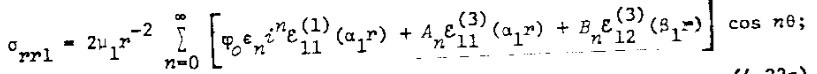
\includegraphics[scale=0.5]{srr1}

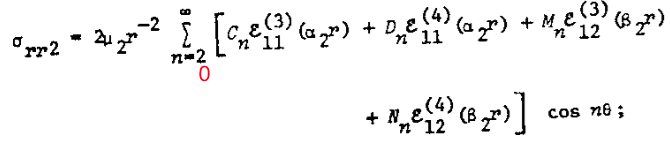
\includegraphics[scale=0.5]{srr2}
\begingroup
\fontsize{10pt}{12pt}
\selectfont
\definecolor{shadecolor}{rgb}{0.925,0.925,0.925}
\begin{shaded}
\begin{verbatim}
      ! sigma_{rr}1 = sigma_{rr}2   @ r = b
      M(1,1) = - muR * e11(3,1,1,2,n)
      M(1,2) = - muR * e12(3,2,1,2,n)
      M(1,3) = e11(3,1,2,2,n)
      M(1,4) = e11(4,1,2,2,n)
      M(1,5) = e12(3,2,2,2,n)
      M(1,6) = e12(4,2,2,2,n) 
      B(1,1) = (1.0) * et(n) * UI**n * muR * e11(1,1,1,2,n)
\end{verbatim}
\end{shaded}
\endgroup
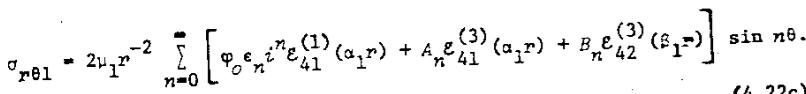
\includegraphics[scale=0.5]{srt1}

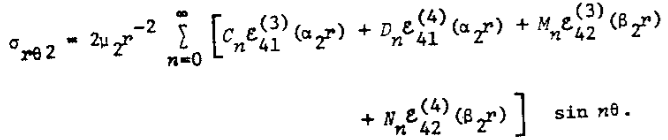
\includegraphics[scale=0.5]{srt2}
\begingroup
\fontsize{10pt}{12pt}
\selectfont
\definecolor{shadecolor}{rgb}{0.925,0.925,0.925}
\begin{shaded}
\begin{verbatim}
      ! sigma_{r th}1 = sigma_{r th}2   @ r = b
      M(2,1) = - muR * e41(3,1,1,2,n)
      M(2,2) = - muR * e42(3,2,1,2,n)
      M(2,3) = e41(3,1,2,2,n)
      M(2,4) = e41(4,1,2,2,n)
      M(2,5) = e42(3,2,2,2,n)
      M(2,6) = e42(4,2,2,2,n)
      B(2,1) = (1.0) * et(n) * UI**n * muR * e41(1,1,1,2,n)

\end{verbatim}
\end{shaded}
\endgroup
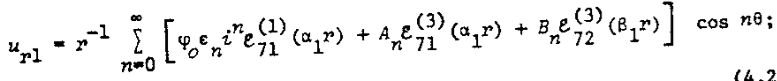
\includegraphics[scale=0.5]{ur1}

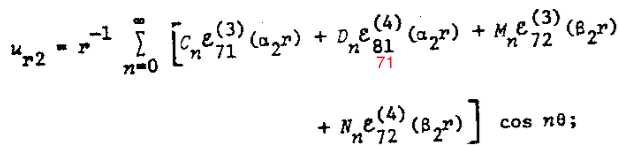
\includegraphics[scale=0.5]{ur2}
\begingroup
\fontsize{10pt}{12pt}
\selectfont
\definecolor{shadecolor}{rgb}{0.925,0.925,0.925}
\begin{shaded}
\begin{verbatim}
      ! u_{r}1 = u_{r}2   @ r = b
      M(3,1) = - e71(3,1,1,2,n) 
      M(3,2) = - e72(3,2,1,2,n) 
      M(3,3) = e71(3,1,2,2,n)
      M(3,4) = e71(4,1,2,2,n) 
      M(3,5) = e72(3,2,2,2,n)
      M(3,6) = e72(4,2,2,2,n)
      B(3,1) = (1.0) * et(n) * UI**n * e71(1,1,1,2,n)
\end{verbatim}
\end{shaded}
\endgroup
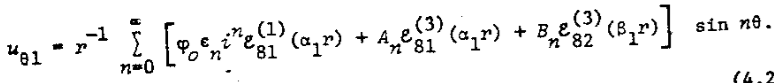
\includegraphics[scale=0.5]{ut1}

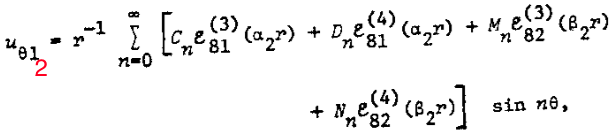
\includegraphics[scale=0.5]{ut2}
\begingroup
\fontsize{10pt}{12pt}
\selectfont
\definecolor{shadecolor}{rgb}{0.925,0.925,0.925}
\begin{shaded}
\begin{verbatim}
      ! u_{th}1 = u_{th}2   @ r = b
      M(4,1) = - e81(3,1,1,2,n) 
      M(4,2) = - e82(3,2,1,2,n) 
      M(4,3) = e81(3,1,2,2,n) 
      M(4,4) = e81(4,1,2,2,n) 
      M(4,5) = e82(3,2,2,2,n)
      M(4,6) = e82(4,2,2,2,n)
      B(4,1) = (1.0) * et(n) * UI**n * e81(1,1,1,2,n)
\end{verbatim}
\end{shaded}
\endgroup
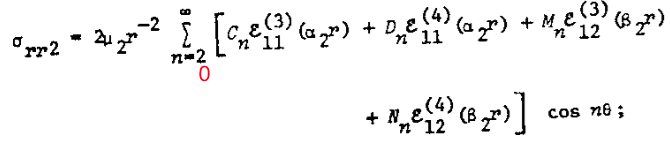
\includegraphics[scale=0.5]{srr2}
\begingroup
\fontsize{10pt}{12pt}
\selectfont
\definecolor{shadecolor}{rgb}{0.925,0.925,0.925}
\begin{shaded}
\begin{verbatim}
      ! sigma_{rr}2 = 0   @ r = a
      M(5,1) = z0
      M(5,2) = z0
      M(5,3) = e11(3,1,2,1,n)
      M(5,4) = e11(4,1,2,1,n)
      M(5,5) = e12(3,2,2,1,n)
      M(5,6) = e12(4,2,2,1,n)
      B(5,1) = z0
\end{verbatim}
\end{shaded}
\endgroup
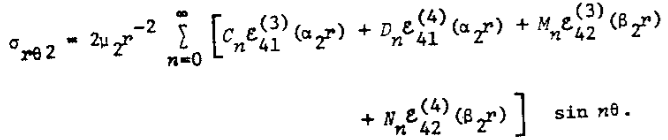
\includegraphics[scale=0.5]{srt2}
\begingroup
\fontsize{10pt}{12pt}
\selectfont
\definecolor{shadecolor}{rgb}{0.925,0.925,0.925}
\begin{shaded}
\begin{verbatim}
      ! sigma_{r th}2 = 0   @ r = a
      M(6,1) = z0
      M(6,2) = z0
      M(6,3) = e41(3,1,2,1,n)
      M(6,4) = e41(4,1,2,1,n)
      M(6,5) = e42(3,2,2,1,n)
      M(6,6) = e42(4,2,2,1,n)
      B(6,1) = z0

\end{verbatim}
\end{shaded}
\endgroup
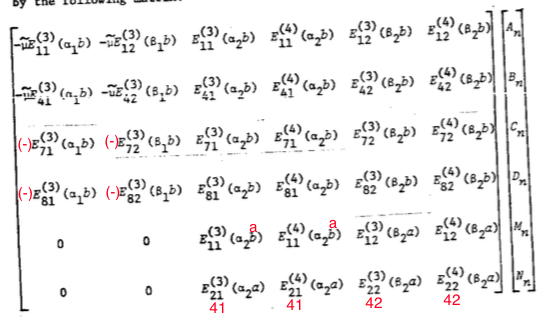
\includegraphics[scale=0.6]{matriz}
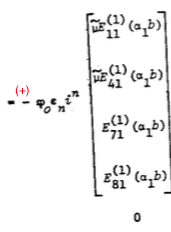
\includegraphics[scale=0.6]{termindep}
\begingroup
\fontsize{10pt}{12pt}
\selectfont
\definecolor{shadecolor}{rgb}{0.925,0.925,0.925}
\begin{shaded}
\begin{verbatim}
!#< r  solve system       . . !#>
      ! driver simple
      call zgesv(6,1,M(1:6,1:6),6,IPIV,B(:,1),6,info)
      
      ! driver experto:
!     call ZGESVX('E','N',6,1,M,6,AF,6,IPIV,EQUED,Rbem, &
!     Cbem,B,6,Xbem,6,RCOND,FERR,BERR,WORKbem,RWORK,INFO)
      
      if(info .ne. 0) then
        write(6,'(A,I0,a,I0)', ADVANCE = "NO") &
        "/",n, " info =",info
        if (info .gt. 6) write(6,'(A)', ADVANCE = "NO") " working precision"
        if (info .le. 6) write(6,'(A)', ADVANCE = "NO") "factor U is exactly singular"
!       stop 1120
        exit
!     else if (abs(B(1,1)) .lt. 0.00000001) then  !NaN
!      write(6,'(A,I0,a)', ADVANCE = "NO") &
!     "trim at",n, " por chiquito abs(B(1)) < 10^{-8}"
!      exit
      else
        write(6,'(A)', ADVANCE = "NO") "."
      end if
!     call showMNmatrixZ(6,1,B,"  A  ",6)     
\end{verbatim}
\end{shaded}
\endgroup

\begingroup
\fontsize{10pt}{12pt}
\selectfont
\definecolor{shadecolor}{rgb}{0.925,0.925,0.925}
\begin{shaded}
\begin{verbatim}
      !#< r elementos mecanicos !#>
      do i = 1,nRes
!      r => Rw(i)%r
       ir = Rw(i)%ir
       th => Rw(i)%th
       reg => Rw(i)%reg
        if (reg .eq. 1) then  !reg 1 in the medium
          Rw(i)%s_rr(J) = Rw(i)%s_rr(J) + &
          (1. * et(n) * UI**n * e11(1,1,1,ir,n) + &
                       B(1,1) * e11(3,1,1,ir,n) + &
                       B(2,1) * e12(3,2,1,ir,n)) * (cos(n * th))
          Rw(i)%s_tt(J) = Rw(i)%s_tt(J) + &
          (1. * et(n) * UI**n * e21(1,1,1,ir,n) + & 
                       B(1,1) * e21(3,1,1,ir,n) + & 
                       B(2,1) * e22(3,2,1,ir,n)) * (cos(n * th))
          Rw(i)%s_rt(J) = Rw(i)%s_rt(J) + &
          (1. * et(n) * UI**n * e41(1,1,1,ir,n) + & 
                       B(1,1) * e41(3,1,1,ir,n) + & 
                       B(2,1) * e42(3,2,1,ir,n)) * (sin(n * th))
          Rw(i)%u_r(J) = Rw(i)%u_r(J) + &
          (1. * et(n) * UI**n * e71(1,1,1,ir,n) + & 
                       B(1,1) * e71(3,1,1,ir,n) + & 
                       B(2,1) * e72(3,2,1,ir,n)) * (cos(n * th))
          Rw(i)%u_t(J) = Rw(i)%u_t(J) + &
          (1. * et(n) * UI**n * e81(1,1,1,ir,n) + & 
                       B(1,1) * e81(3,1,1,ir,n) + & 
                       B(2,1) * e82(3,2,1,ir,n)) * (sin(n * th))
        else if (reg .eq. 2) then !reg 2 in the lining
          Rw(i)%s_rr(J) = Rw(i)%s_rr(J) + &
                      (B(3,1) * e11(3,1,2,ir,n) + &
                       B(4,1) * e11(4,1,2,ir,n) + &
                       B(5,1) * e12(3,2,2,ir,n) + &
                       B(6,1) * e12(4,2,2,ir,n)) * (cos(n * th))
          Rw(i)%s_tt(J) = Rw(i)%s_tt(J) + &
                      (B(3,1) * e21(3,1,2,ir,n) + &
                       B(4,1) * e21(4,1,2,ir,n) + &
                       B(5,1) * e22(3,2,2,ir,n) + &
                       B(6,1) * e22(4,2,2,ir,n)) * (cos(n * th))
          Rw(i)%s_rt(J) = Rw(i)%s_rt(J) + &
                      (B(3,1) * e41(3,1,2,ir,n) + &
                       B(4,1) * e41(4,1,2,ir,n) + &
                       B(5,1) * e42(3,2,2,ir,n) + &
                       B(6,1) * e42(4,2,2,ir,n)) * (sin(n * th))
          Rw(i)%u_r(J) = Rw(i)%u_r(J) + &
                      (B(3,1) * e71(3,1,2,ir,n) + &
                       B(4,1) * e71(4,1,2,ir,n) + &
                       B(5,1) * e72(3,2,2,ir,n) + &
                       B(6,1) * e72(4,2,2,ir,n)) * (cos(n * th))
          Rw(i)%u_t(J) = Rw(i)%u_t(J) + &
                      (B(3,1) * e81(3,1,2,ir,n) + &
                       B(4,1) * e81(4,1,2,ir,n) + &
                       B(5,1) * e82(3,2,2,ir,n) + &
                       B(6,1) * e82(4,2,2,ir,n)) * (sin(n * th))
        end if
      end do! i:nRes
      end do !n
      
      ! términos fuera de la suma:
      do i = 1,nRes
       r => Rw(i)%r
!      th => Rw(i)%th
       reg => Rw(i)%reg
       sig0 = amu(1) * beta(1)**2. !eq 3.15   para hacerlo factor de amplificación
          Rw(i)%s_rr(J) = Rw(i)%s_rr(J) * 2. *amu(reg) / r**2. 
          Rw(i)%s_tt(J) = Rw(i)%s_tt(J) * 2. *amu(reg) / r**2. !/ sig0
          Rw(i)%s_rt(J) = Rw(i)%s_rt(J) * 2. *amu(reg) / r**2. 
          Rw(i)%u_r(J) = Rw(i)%u_r(J) / r 
          Rw(i)%u_t(J) = Rw(i)%u_t(J) / r 
      end do! i:nRes

\end{verbatim}
\end{shaded}
\endgroup

\begingroup
\fontsize{10pt}{12pt}
\selectfont
\definecolor{shadecolor}{rgb}{0.925,0.925,0.925}
\begin{shaded}
\begin{verbatim}
      abscisa(J) = dfrec * 2 * pi * J * radios(1) / cp(1)
      end do !J   
      ! plot curves
      ! end program tunelRecub
      print*,"printing"
      
      
      
      
      
      
      
      
      
      
      
      
      
      
      
      
      
      
      
      
      
      
      
      
      
      
      
      
      
      
      
      
      
      
      
      
      
      
\end{verbatim}
\end{shaded}
\endgroup
Se comparan los resultados normalizados para $\eta=1.1$, $r=b$,

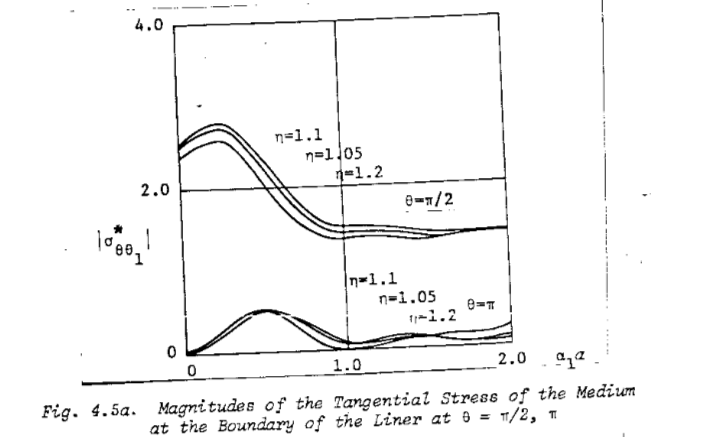
\includegraphics[scale=0.4]{res1}

en $\theta=\pi/2$ y en $\theta=\pi$ respectivamente,

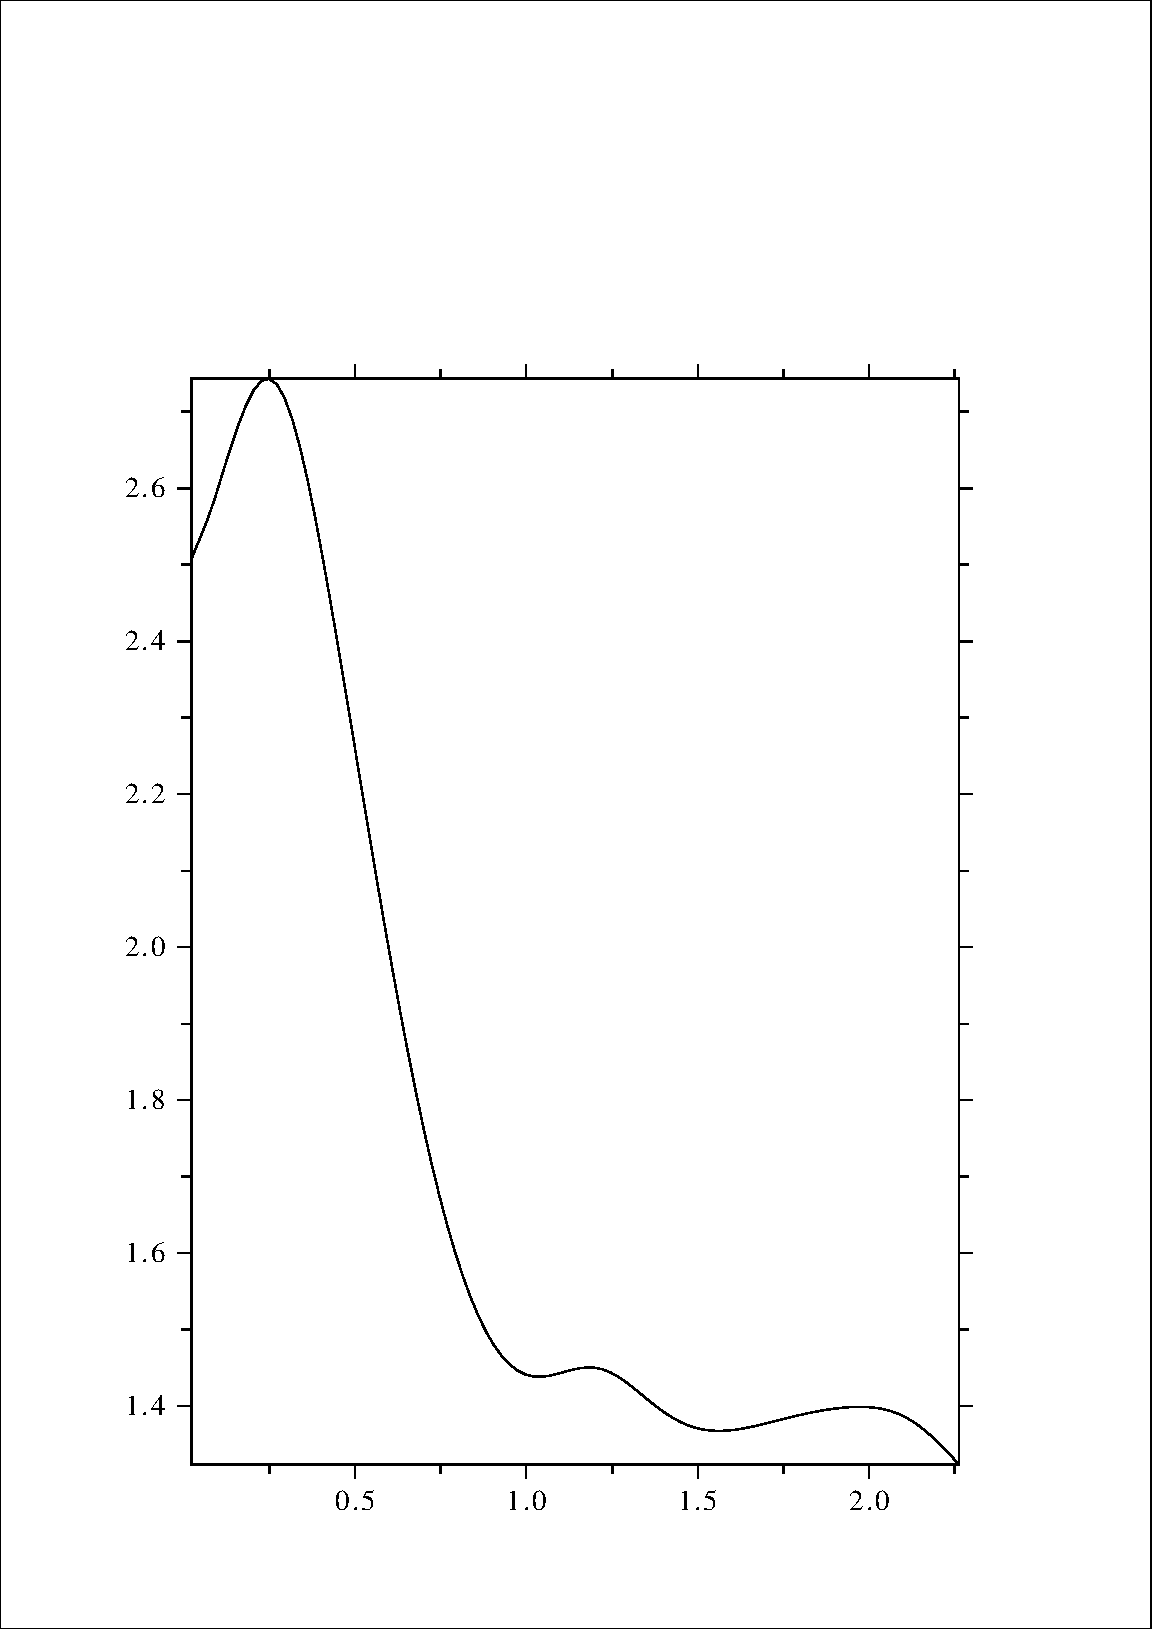
\includegraphics[scale=0.4]{RES_1s_tt1abspi2.pdf}
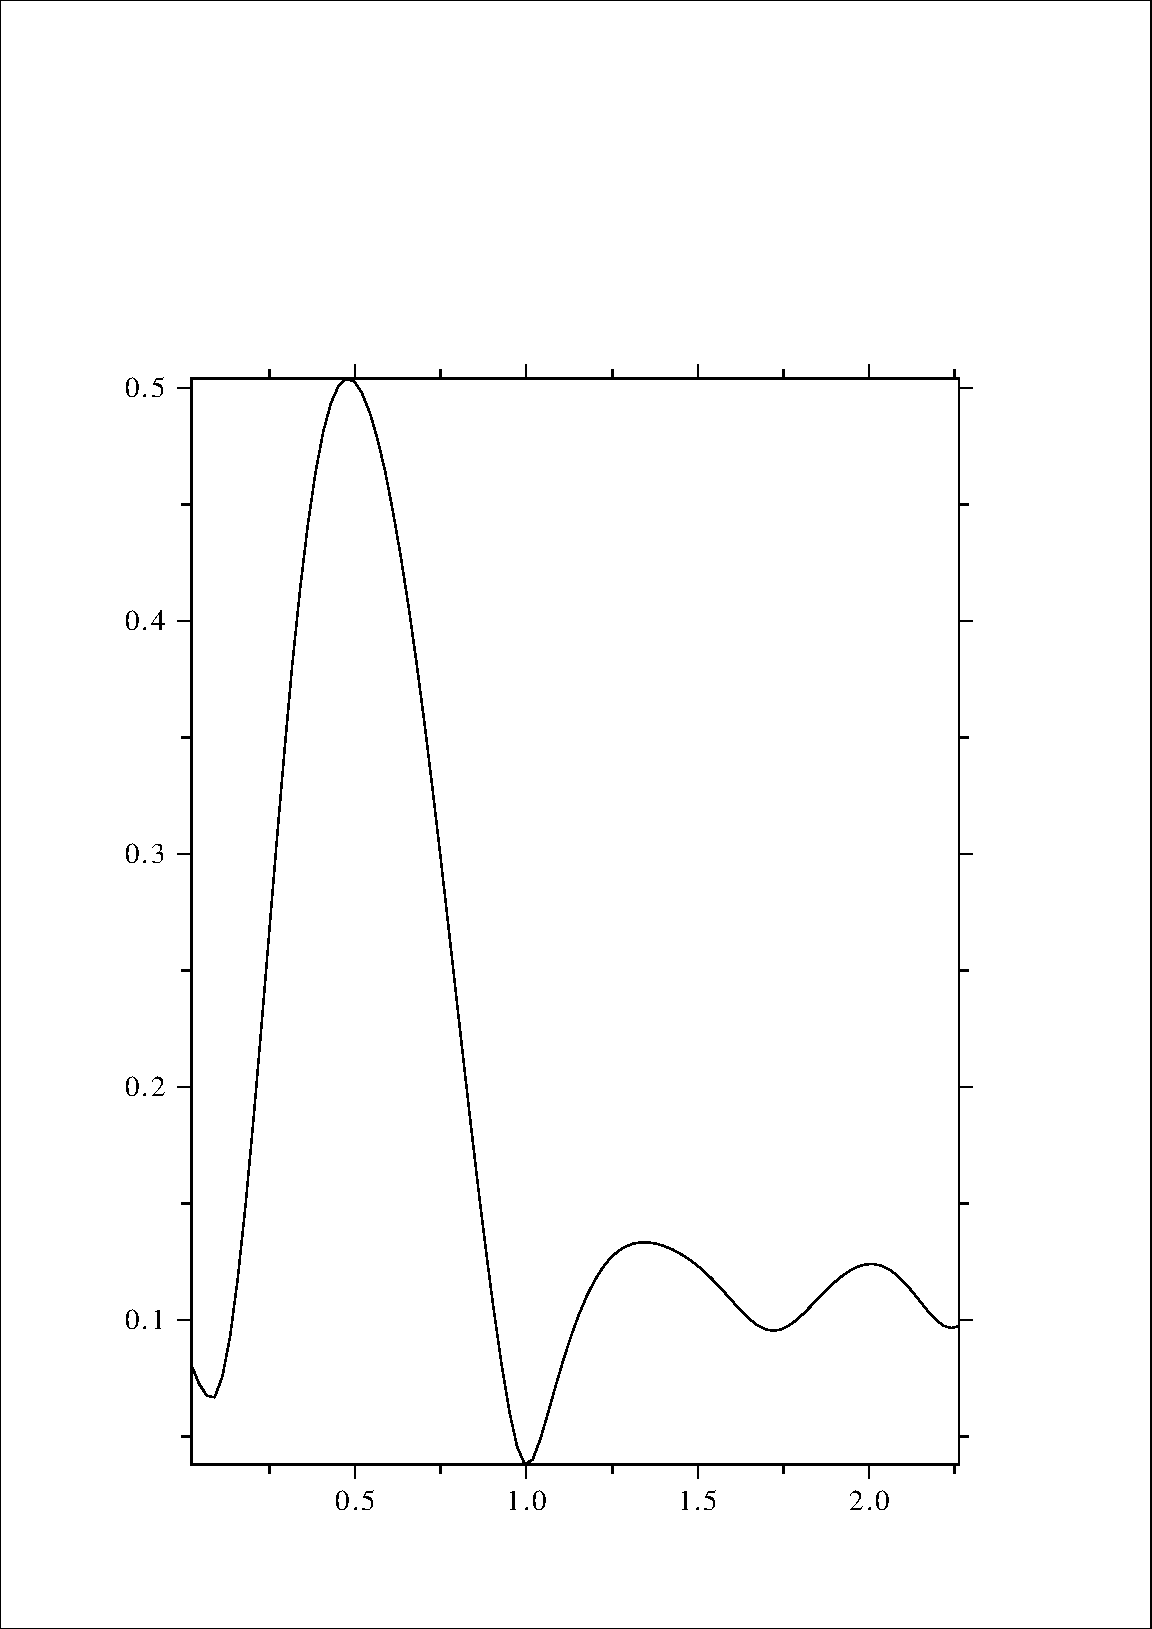
\includegraphics[scale=0.4]{RES_1s_tt1abspi.pdf}

y en $\eta=1.1$, $r=a$, 

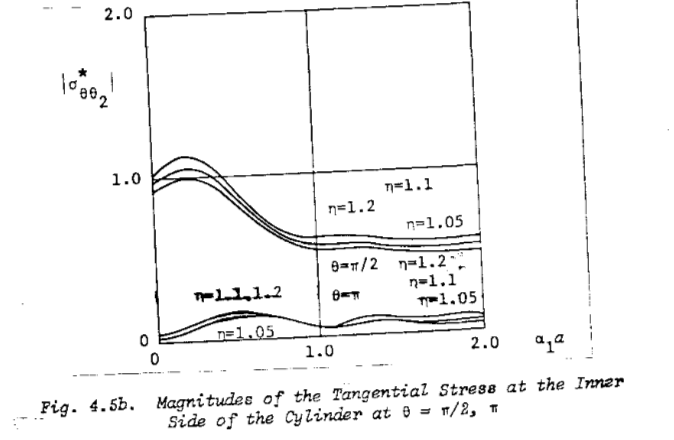
\includegraphics[scale=0.4]{res2}

en $\theta=\pi/2$ y en $\theta=\pi$ respectivamente,

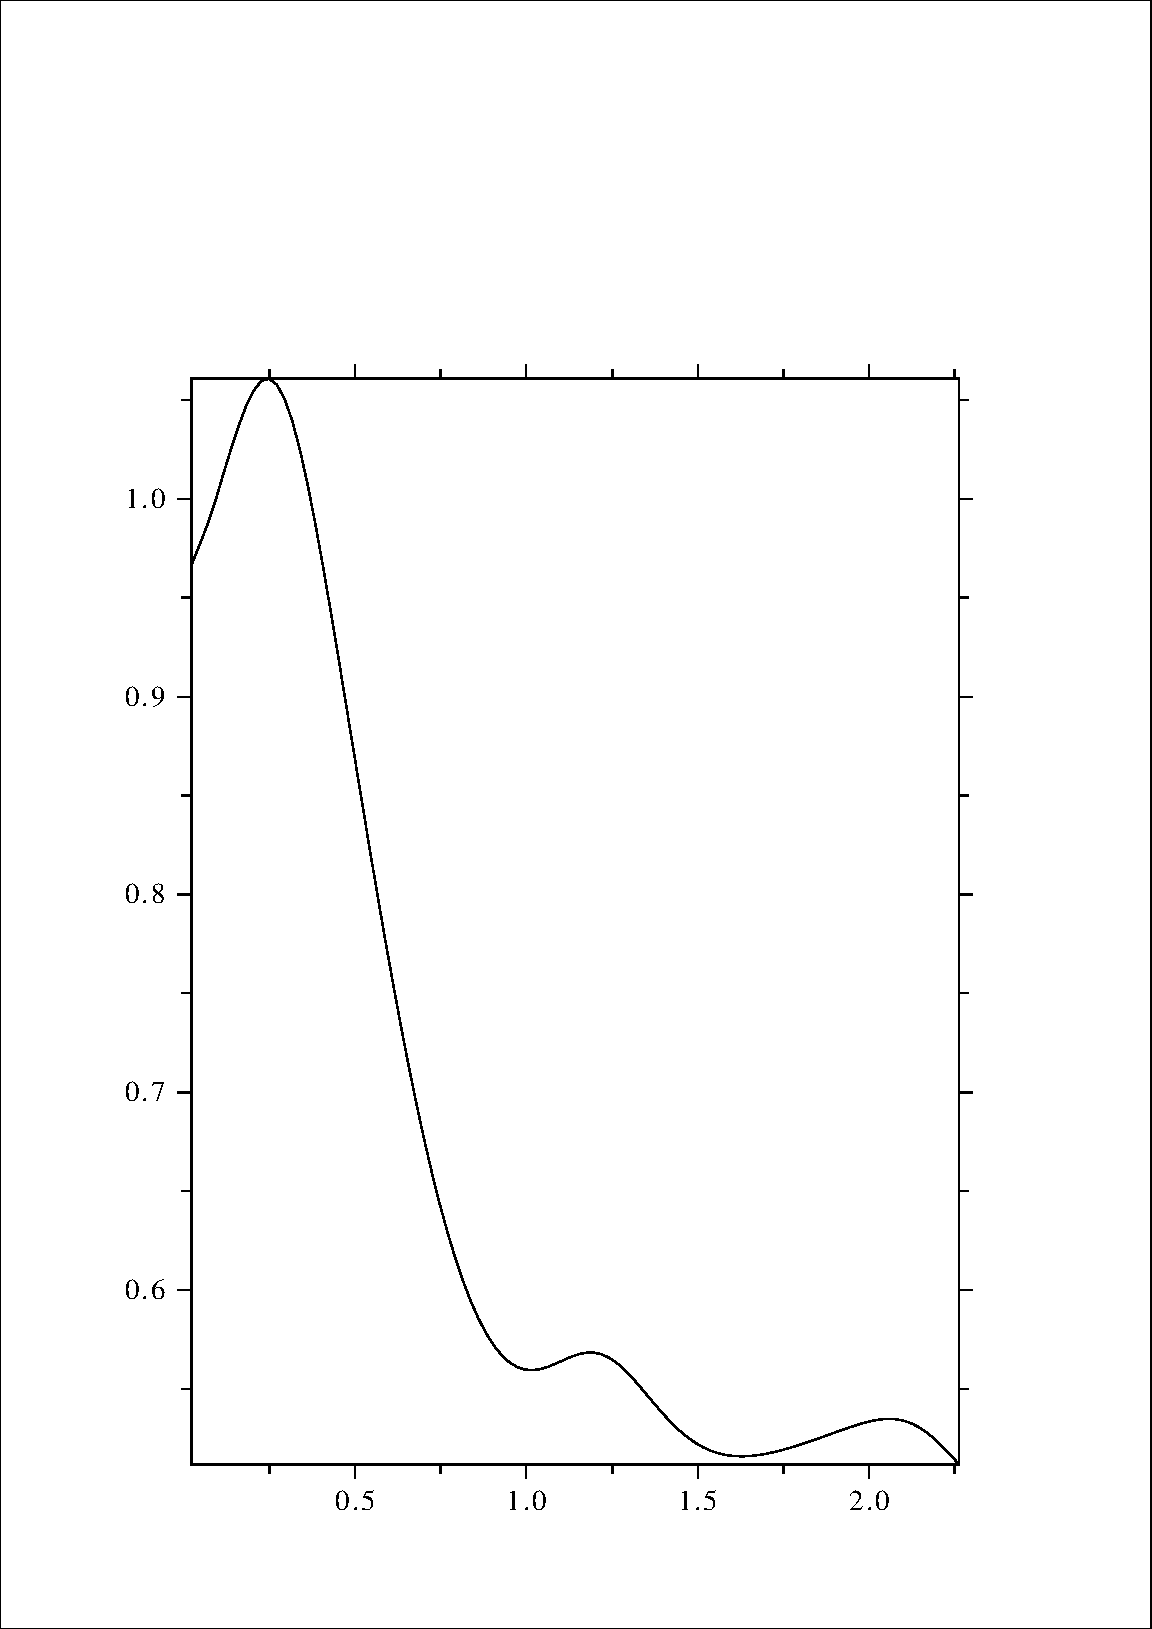
\includegraphics[scale=0.4]{RES_2s_tt2abspi2.pdf}
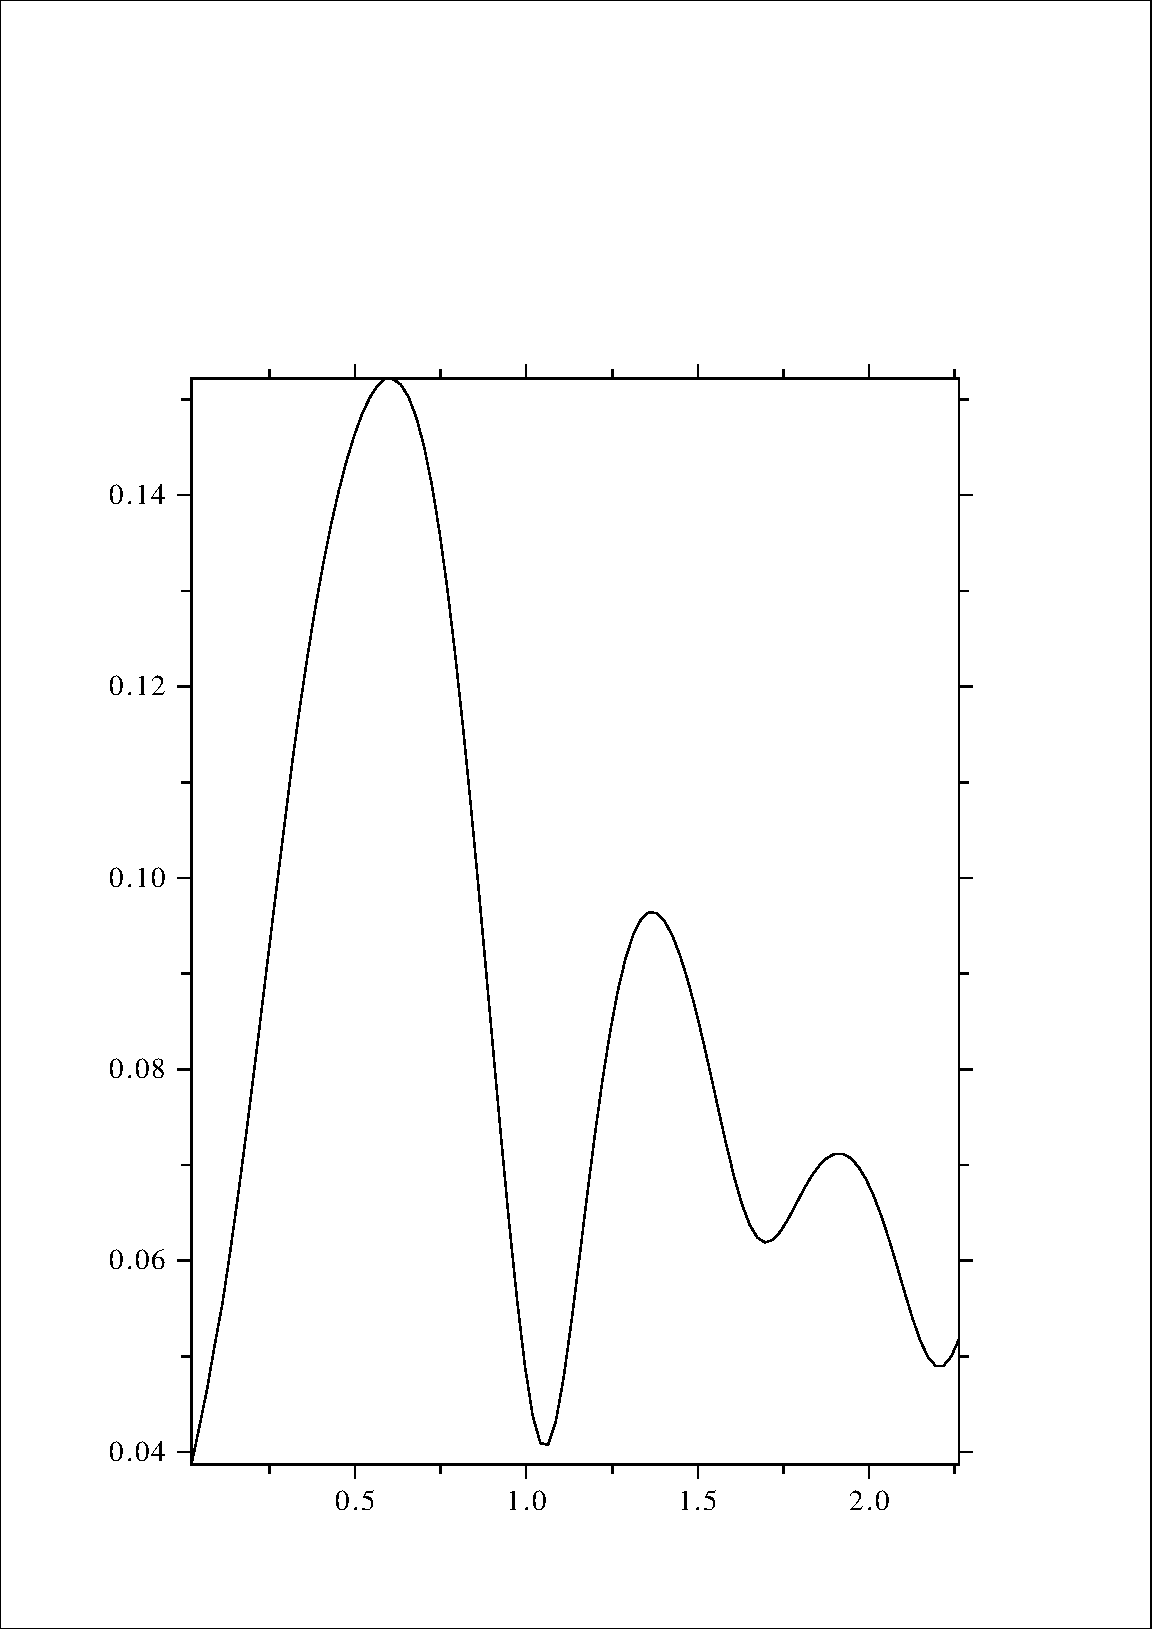
\includegraphics[scale=0.4]{RES_2s_tt2abspi.pdf}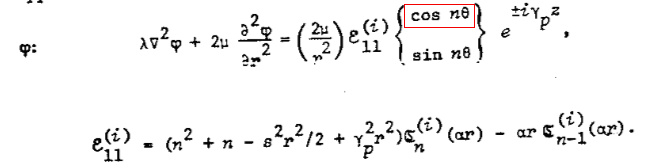
\includegraphics[scale=0.5]{e11}
\begingroup
\fontsize{10pt}{12pt}
\selectfont
\definecolor{shadecolor}{rgb}{0.925,0.925,0.925}
\begin{shaded}
\begin{verbatim}
      function e11(i,c,reg,r,n)
      use vars_func_of_w, only : alfa,s2,gammaP
      use datos, only : radios
      use Hank, only : Bess
      implicit none
      complex*16 :: e11
      integer :: i,c,reg,r,n
      complex*16, pointer :: Bess_n,Bess_n_1
!     c = 1 !alfa
      Bess_n => Bess(reg)%JYH1H2(i,n)%r(r)%c(1)
      Bess_n_1 => Bess(reg)%JYH1H2(i,n-1)%r(r)%c(1)
      e11 = (n**2 + n - s2(reg) * radios(r)**2 / 2. + & 
      gammaP**2 * radios(r)**2) * Bess_n - alfa(reg)* radios(r) * Bess_n_1
      end function e11
\end{verbatim}
\end{shaded}
\endgroup
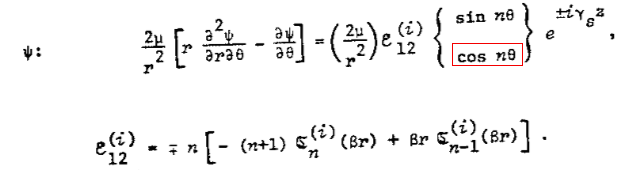
\includegraphics[scale=0.5]{e12}
\begingroup
\fontsize{10pt}{12pt}
\selectfont
\definecolor{shadecolor}{rgb}{0.925,0.925,0.925}
\begin{shaded}
\begin{verbatim}
      function e12(i,c,reg,r,n)
      use vars_func_of_w, only : beta
      use datos, only : radios
      use Hank, only : Bess
      implicit none
      complex*16 :: e12
      integer :: i,c,reg,r,n
      complex*16, pointer :: Bess_n,Bess_n_1
!     c = 2 !beta
      Bess_n => Bess(reg)%JYH1H2(i,n)%r(r)%c(2)
      Bess_n_1 => Bess(reg)%JYH1H2(i,n-1)%r(r)%c(2)
      e12 = n * (-(n+1)* Bess_n + beta(reg) * radios(r) * Bess_n_1)
      end function e12
\end{verbatim}
\end{shaded}
\endgroup
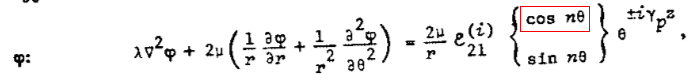
\includegraphics[scale=0.5]{e21a}

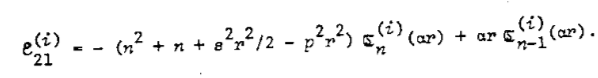
\includegraphics[scale=0.5]{e21b}
\begingroup
\fontsize{10pt}{12pt}
\selectfont
\definecolor{shadecolor}{rgb}{0.925,0.925,0.925}
\begin{shaded}
\begin{verbatim}
      function e21(i,c,reg,r,n)
      use vars_func_of_w, only : alfa,s2,p2
      use datos, only : radios
      use Hank, only : Bess
      implicit none
      complex*16 :: e21
      integer :: i,c,reg,r,n
      complex*16, pointer :: Bess_n,Bess_n_1
!     c = 1 !alfa
      Bess_n => Bess(reg)%JYH1H2(i,n)%r(r)%c(1)
      Bess_n_1 => Bess(reg)%JYH1H2(i,n-1)%r(r)%c(1)
      e21 = - (n**2 + n + s2(reg)*radios(r)**2 / 2. - p2(reg)*radios(r)**2) * &
             Bess_n + alfa(reg) * radios(r) * Bess_n_1
      end function e21
\end{verbatim}
\end{shaded}
\endgroup
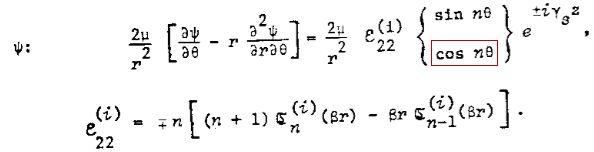
\includegraphics[scale=0.5]{e22}
\begingroup
\fontsize{10pt}{12pt}
\selectfont
\definecolor{shadecolor}{rgb}{0.925,0.925,0.925}
\begin{shaded}
\begin{verbatim}
      function e22(i,c,reg,r,n)
      use vars_func_of_w, only : beta
      use datos, only : radios
      use Hank, only : Bess
      implicit none
      complex*16 :: e22
      integer :: i,c,reg,r,n
      complex*16, pointer :: Bess_n,Bess_n_1
!     c = 2 !beta
      Bess_n => Bess(reg)%JYH1H2(i,n)%r(r)%c(2)
      Bess_n_1 => Bess(reg)%JYH1H2(i,n-1)%r(r)%c(2)
      e22 = n * ((n+1)*Bess_n - beta(reg)*radios(r)*Bess_n_1)
      end function e22
\end{verbatim}
\end{shaded}
\endgroup
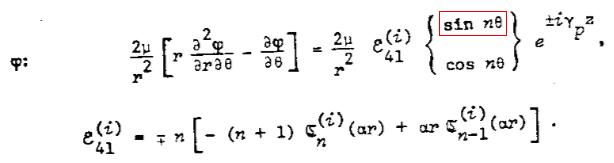
\includegraphics[scale=0.5]{e41}
\begingroup
\fontsize{10pt}{12pt}
\selectfont
\definecolor{shadecolor}{rgb}{0.925,0.925,0.925}
\begin{shaded}
\begin{verbatim}
      function e41(i,c,reg,r,n)
      use vars_func_of_w, only : alfa
      use datos, only : radios
      use Hank, only : Bess
      implicit none
      complex*16 :: e41
      integer :: i,c,reg,r,n
      complex*16, pointer :: Bess_n,Bess_n_1
!     c = 1 !alfa
      Bess_n => Bess(reg)%JYH1H2(i,n)%r(r)%c(1)
      Bess_n_1 => Bess(reg)%JYH1H2(i,n-1)%r(r)%c(1)
      e41 = - n * (-(n+1) * Bess_n + alfa(reg)*radios(r)*Bess_n_1)
      end function e41
\end{verbatim}
\end{shaded}
\endgroup
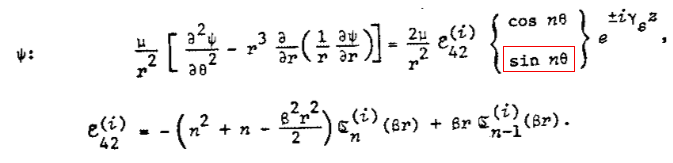
\includegraphics[scale=0.5]{e42}
\begingroup
\fontsize{10pt}{12pt}
\selectfont
\definecolor{shadecolor}{rgb}{0.925,0.925,0.925}
\begin{shaded}
\begin{verbatim}
      function e42(i,c,reg,r,n)
      use vars_func_of_w, only : beta
      use datos, only : radios
      use Hank, only : Bess
      implicit none
      complex*16 :: e42
      integer :: i,c,reg,r,n
      complex*16, pointer :: Bess_n,Bess_n_1
!     c = 2 !beta
      Bess_n => Bess(reg)%JYH1H2(i,n)%r(r)%c(2)
      Bess_n_1 => Bess(reg)%JYH1H2(i,n-1)%r(r)%c(2)
      e42 = - (n**2 + n - beta(reg)**2 * radios(r)**2 / 2.) * Bess_n + &
            beta(reg) * radios(r) * Bess_n_1
      end function e42
\end{verbatim}
\end{shaded}
\endgroup
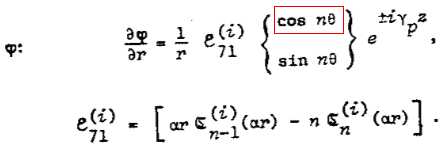
\includegraphics[scale=0.5]{e71}
\begingroup
\fontsize{10pt}{12pt}
\selectfont
\definecolor{shadecolor}{rgb}{0.925,0.925,0.925}
\begin{shaded}
\begin{verbatim}
      function e71(i,c,reg,r,n)
      use vars_func_of_w, only : alfa
      use datos, only : radios
      use Hank, only : Bess
      implicit none
      complex*16 :: e71
      integer :: i,c,reg,r,n
      complex*16, pointer :: Bess_n,Bess_n_1
!     c = 1 !alfa
      Bess_n => Bess(reg)%JYH1H2(i,n)%r(r)%c(1)
      Bess_n_1 => Bess(reg)%JYH1H2(i,n-1)%r(r)%c(1)
      e71 = alfa(reg) * radios(r) * Bess_n_1 - n * Bess_n
      end function e71
\end{verbatim}
\end{shaded}
\endgroup
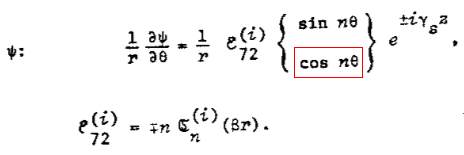
\includegraphics[scale=0.5]{e72}
\begingroup
\fontsize{10pt}{12pt}
\selectfont
\definecolor{shadecolor}{rgb}{0.925,0.925,0.925}
\begin{shaded}
\begin{verbatim}
      function e72(i,c,reg,r,n)
      use Hank, only : Bess
      implicit none
      complex*16 :: e72
      integer :: i,c,reg,r,n
      complex*16, pointer :: Bess_n
!     c = 2 !beta
      Bess_n => Bess(reg)%JYH1H2(i,n)%r(r)%c(2)
      e72 = n * Bess_n
      end function e72
\end{verbatim}
\end{shaded}
\endgroup
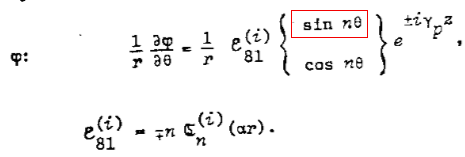
\includegraphics[scale=0.5]{e81}
\begingroup
\fontsize{10pt}{12pt}
\selectfont
\definecolor{shadecolor}{rgb}{0.925,0.925,0.925}
\begin{shaded}
\begin{verbatim}
      function e81(i,c,reg,r,n)
      use Hank, only : Bess
      implicit none
      complex*16 :: e81
      integer :: i,c,reg,r,n
      complex*16, pointer :: Bess_n
!     c = 1 !alfa
      Bess_n => Bess(reg)%JYH1H2(i,n)%r(r)%c(1)
      e81 = - n * Bess_n
      end function e81
\end{verbatim}
\end{shaded}
\endgroup
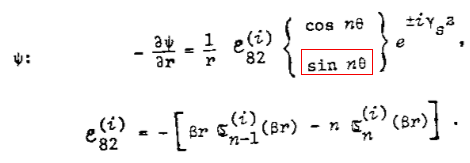
\includegraphics[scale=0.5]{e82}
\begingroup
\fontsize{10pt}{12pt}
\selectfont
\definecolor{shadecolor}{rgb}{0.925,0.925,0.925}
\begin{shaded}
\begin{verbatim}
      function e82(i,c,reg,r,n)
      use vars_func_of_w, only : beta
      use datos, only : radios
      use Hank, only : Bess
      implicit none
      complex*16 :: e82
      integer :: i,c,reg,r,n
      complex*16, pointer :: Bess_n,Bess_n_1
!     c = 2 !beta
      Bess_n => Bess(reg)%JYH1H2(i,n)%r(r)%c(2)
      Bess_n_1 => Bess(reg)%JYH1H2(i,n-1)%r(r)%c(2)
      e82 = - (beta(reg) * radios(r) * Bess_n_1 & 
              - n * Bess_n)
      end function e82
\end{verbatim}
\end{shaded}
\endgroup

\end{document}
